%%%%%%%%%%%%%%%%%%%%%%%%%%%%%%%%%%%%

\section{6.5. Inferência para uma proporção com uma amostra pequena}

%%%%%%%%%%%%%%%%%%%%%%%%%%%%%%%%%%%%

\subsection{Paul, o polvo}

%%%%%%%%%%%%%%%%%%%%%%%%%%%%%%%%%%%%

\begin{frame}
\frametitle{Preditores famosos}

\twocol{0.5}{0.5}{
Antes desse cara...
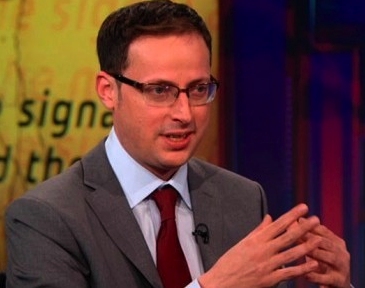
\includegraphics[width=\textwidth]{6-5_small_single_prop/nate.png}
}
{
\pause
Tinha esse cara...
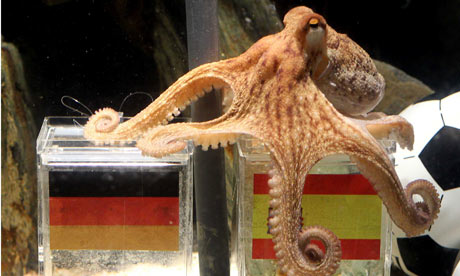
\includegraphics[width=\textwidth]{6-5_small_single_prop/paul.png}
}

\end{frame}

%%%%%%%%%%%%%%%%%%%%%%%%%%%%%%%%%%

\begin{frame}
\frametitle{Paul, o polvo - psíquico?}

\begin{itemize}
\justifying
\item Paul, o polvo, previu 8 jogos da Copa do Mundo corretamente.

\pause
\justifying
\item Isso fornece evidências convincentes de que Paul realmente tem poderes psíquicos?

\pause
\justifying
\item Quão incomum seria se ele estivesse apenas adivinhando aleatoriamente (com 50\% de chance de
adivinhar corretamente)?

\pause
\justifying
\item Hipóteses:
\begin{itemize}
\item[$H_0:$] $p = 0.5$
\item[$H_A:$] $p > 0.5$
\end{itemize}

\end{itemize}

\end{frame}

%%%%%%%%%%%%%%%%%%%%%%%%%%%%%%%%%%

\begin{frame}
\frametitle{Condições}

\begin{enumerate}
\justifying
\item \hl{Independência:} Podemos supor que cada palpite é independente de outro.

\pause
\justifying
\item \hl{Tamanho da amostra:} O número de sucessos esperados é \orange{menor que 10}.
\[ 8 \times 0.5 = 4 \]

\end{enumerate}

\pause

\vspace{1cm}
\justifying
\dq{Então, o que fazemos?}

\pause
\justifying
Como o tamanho da amostra não é grande o suficiente para usar métodos baseados em TCL, usamos um método de simulação.

\end{frame}

%%%%%%%%%%%%%%%%%%%%%%%%%%%%%%%%%%

\begin{frame}
\frametitle{Prática}
\justifying
\pq{Qual dos seguintes métodos é a melhor maneira de calcular o p-valor do teste de hipótese para testar se as previsões de Paul, o polvo, são excepcionalmente mais altas do que adivinhações aleatórias?}

\scalefont{0.8}
\begin{enumerate}[(a)]
\justifying
\item Jogue uma moeda 8 vezes, registre a proporção de vezes em que todos os 8 lançamentos foram cara. Repita isso muitas vezes e calcule a proporção de simulações em que todos os 8 lançamentos foram cara.
\justifying
\item Jogue um dado 8 vezes, registre a proporção de vezes em que todos os 8 lançamentos foram 6s. Repita isso várias vezes e calcule a proporção de simulações em que todos os 8 lançamentos foram 6s.
\justifying
\item Jogue uma moeda 10.000 vezes, registre a proporção de cara. Repita isso várias vezes e calcule a proporção de simulações em que mais de 50\% dos lançamentos são cara.
\justifying
\item Jogue uma moeda 10.000 vezes, calcule a proporção de cara.
\end{enumerate}

\end{frame}

%%%%%%%%%%%%%%%%%%%%%%%%%%%%%%%%%%%

\begin{frame}
\frametitle{Simular}
\justifying
\pq{Jogue uma moeda 8 vezes. Você conseguiu todas as caras?}

\begin{enumerate}[(a)]
\item Sim
\item Não
\end{enumerate}

\end{frame}

%%%%%%%%%%%%%%%%%%%%%%%%%%%%%%%%%%

\begin{frame}[fragile]
\frametitle{Simular}
\justifying
{\tiny
\begin{Verbatim}[frame=single, formatcom=\color{blue}]
fonte ("http://www.openintro.org/stat/slides/inference.R")
paul = fator(c(rep("sim", 8), rep("não", 0)), nível = c("sim","não"))
inferência(paul, est = "proporção", tipo = "ht", método = "simulação",
          sucesso = "sim", nulo = 0.5, alternativo = "maior", semente = 290)
\end{Verbatim}
}

\pause
\justifying
{\tiny
\begin{Verbatim}[frame=single, formatcom=\color{gray}]
Proporção única -- sucesso: sim
Estatísticas resumidas: p_hat = 1 ;  n = 8 
H0: p = 0.5 
HA: p > 0.5 
valor-p =  0.0037
\end{Verbatim}
}

\centering
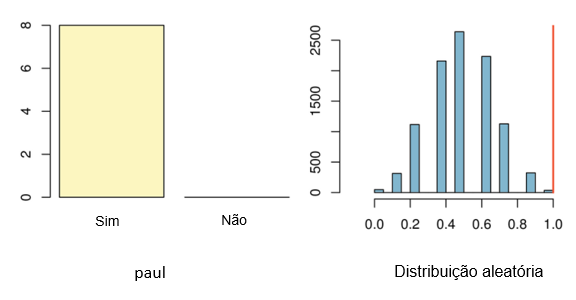
\includegraphics[width=0.8\textwidth,height=0.4\textheight]{6-5_small_single_prop/paul_HT.png}

\end{frame}

%%%%%%%%%%%%%%%%%%%%%%%%%%%%%%%%%%%

\begin{frame}
\frametitle{Conclusões}
\justifying
\pq{Qual das seguintes opções é \underline {falsa}??}

\begin{enumerate}[(a)]
\justifying
\item Se, de fato, Paul estivesse adivinhando aleatoriamente, a probabilidade de ele obter o resultado de todos os 8 jogos corretos é 0,0037.
\justifying
\item Rejeitar $H_0$, os dados fornecem evidências convincentes de que Paul fez mais do que adivinhar aleatoriamente.
\justifying
\item Podemos ter cometido um erro do Tipo I.

\solnMult{A probabilidade de que Paul seja psíquico é 0,0037.}

\end{enumerate}

\end{frame}

%%%%%%%%%%%%%%%%%%%%%%%%%%%%%%%%%%%%

\subsection{Dorso da mão}

%%%%%%%%%%%%%%%%%%%%%%%%%%%%%%%%%%%

\begin{frame}
\frametitle{Dorso da mão}
\justifying
\dq{Há um ditado que diz "conheça algo como a palma da sua mão". Descreva um experimento para testar se as pessoas conhecem \textit{o dorso} de suas mãos.}

\pause

\begin{center}
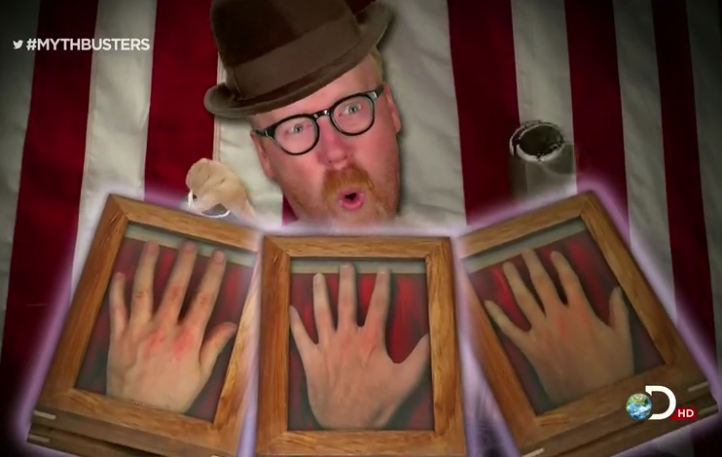
\includegraphics[width=0.6\textwidth]{6-5_small_single_prop/mythbusters.png}
\end{center}
\justifying
No episódio de MythBusters, 11 de 12 pessoas adivinham as costas de suas mãos corretamente.

\end{frame}

%%%%%%%%%%%%%%%%%%%%%%%%%%%%%%%%%%%%

\begin{frame}
\frametitle{Hipóteses}
\justifying
\dq{Quais são as hipóteses para avaliar se as pessoas são capazes de reconhecer o dorso da mão a uma taxa melhor que uma adivinhação aleatória. Lembre-se, no experimento do MythBusters, havia 10 fotos para escolher, e apenas 1 estava correta.}

\begin{itemize}
\item[$H_0:$] $p = 0.10$ (adivinhação aleatória)
\item[$H_A:$] $p > 0.10$ (mais do que adivinhar aleatoriamente)
\end{itemize}

\end{frame}

%%%%%%%%%%%%%%%%%%%%%%%%%%%%%%%%%%%

\begin{frame}
\frametitle{Condições}

\begin{enumerate}
\justifying
\item \hl{Independência:} Podemos supor que cada pessoa que adivinhando é independente de outra.
\justifying
\item \hl{Tamanho da amostra:} O número de sucessos esperados é \orange{menor que 10}.
\[ 12 \times 0.1 = 1.2 \]

\end{enumerate}
\justifying
\dq{Então, o que fazemos?}
\justifying
Como o tamanho da amostra não é grande o suficiente para usar métodos baseados em TCL, usamos um método de simulação.

\end{frame}

%%%%%%%%%%%%%%%%%%%%%%%%%%%%%%%%%%%

\subsection{Aleatorização HT para uma proporção}

%%%%%%%%%%%%%%%%%%%%%%%%%%%%%%%%%%%%

\begin{frame}
\frametitle{Esquema de simulação}
\justifying
\dq{Descreva como você testaria se os resultados desse experimento determinam se as pessoas são capazes de reconhecer o dorso da mão a uma taxa melhor do que uma adivinhação aleatória.}
\vspace{-0.5cm}
\[ H_0: p = 0.10 \qquad H_A: p > 0.10 \qquad \hat{p} = 11 / 12 = 0.9167 \]

\scalefont{0.7}
\begin{enumerate}
\justifying
\item Use um dado justo de 10 lados para representar o espaço de amostragem, e chame 1 de sucesso (adivinhando corretamente), e todas os outros resultados de falhas (adivinhando incorretamente).

\justifying
\item Jogue o dado 12 vezes (representando 12 pessoas no experimento), conte o número de 1s e calcule a proporção de palpites corretos em uma simulação com 12 lançamentos.
\justifying
\item Repita o passo (2) muitas vezes, registrando a proporção de sucessos em uma série de 12 lançamentos do dado.
\justifying
\item Crie um gráfico de pontos das proporções simuladas a partir do passo (3) e conte o número de simulações em que a proporção foi pelo menos tão alta quanto 0.9167 (a proporção observada).

\end{enumerate}

\end{frame}

%%%%%%%%%%%%%%%%%%%%%%%%%%%%%%%%%%%

\begin{frame}
\frametitle{Resultados simulados}

\begin{itemize}
\justifying
\item No próximo slide você pode ver os resultados de um teste de hipótese (usando apenas 100 simulações para manter as coisas simples).
\justifying
\item Cada ponto representa uma proporção de sucesso da simulação. Houve 25-30 simulações em que a taxa de sucesso ($\hat{p}$) foi de 10\%, 40-45 simulações em que a taxa de sucesso foi ligeiramente inferior a 10\%, cerca de 20 simulações em que a taxa de sucesso foi ligeiramente menor que 20\% e 1 simulação em que a taxa de sucesso foi superior a 30\%.
\justifying
\item Não há simulações em que a taxa de sucesso seja tão alta quanto a taxa de sucesso observada de 91.67\%.

\end{itemize}
\end{frame}

%%%%%%%%%%%%%%%%%%%%%%%%%%%%%%%%%%%

\begin{frame}
\frametitle{Resultados simulados}

\begin{itemize}
\justifying
\item Portanto, concluímos que o resultado observado é quase impossível de acontecer por acaso (p-valor = 0).
\justifying
\item E, portanto, esses dados sugerem que as pessoas são capazes de reconhecer as costas de suas mãos a uma taxa melhor do que adivinhar aleatoriamente.

\end{itemize}

\end{frame}

%%%%%%%%%%%%%%%%%%%%%%%%%%%%%%%%%%%%

\begin{frame}[fragile]
\frametitle{Resultados simulados}
\justifying
{\tiny
\begin{Verbatim}[frame=single, formatcom=\color{blue}]
costas = as.factor(c(rep("correto", 11), rep("errado", 1))) 
inferência(costas, est = "proporção", tipo = "ht", método = "simulação",
	sucesso = "correto", nulo = 0.1, alternativo = "maior", semente = 654, nsim = 100)
\end{Verbatim}
}

\pause
\justifying
{\tiny
\begin{Verbatim}[frame=single, formatcom=\color{gray}]
Proporção única - sucesso: correto 
Estatísticas resumidas: p_hat = 0.9167 ;  n = 12 
H0: p = 0.1 
HA: p > 0.1 
p-value =  0 
\end{Verbatim}
}

\centering
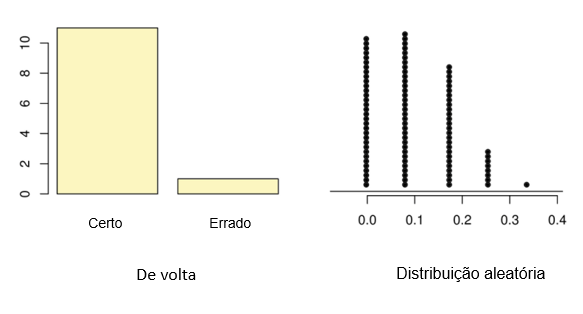
\includegraphics[width=0.8\textwidth,height=0.4\textheight]{6-5_small_single_prop/back_HT.png}

\end{frame}

%%%%%%%%%%%%%%%%%%%%%%%%%%%%%%%%%%%
